%
%  ssrn_analysis.tex
%
%  Created by Drew Conway on 2010-11-29.
% 
%
\documentclass[xcolor=dvipsnames, 9pt]{beamer}

\newenvironment{code}{\begin{semiverbatim} \begin{footnotesize}}
{\end{footnotesize}\end{semiverbatim}}

\usepackage{graphicx}
\usepackage{amssymb}
\usepackage{amsfonts}
\usepackage{amsmath}
\usepackage{hyperref}
\usepackage{natbib}
\usepackage{color}
\usepackage{pdfsync}
\usepackage{chancery}
\usepackage{movie15}
\usepackage{pgfpages}
\usepackage{fancyvrb}
\usepackage{colortbl}

% \definecolor{white}{rgb}{255,255,255}
% \definecolor{darkred}{rgb}{0.5,0,0}
% \definecolor{darkgreen}{rgb}{0,0.5,0}
% \definecolor{lightblue}{rgb}{0,0,0.7}

% \hypersetup{colorlinks,
%   linkcolor=white,
%   filecolor=darkred,
%   urlcolor=lightblue,
%   citecolor=darkblue}

\usepackage{beamerthemesplit}
\usetheme{Warsaw}
\usecolortheme[named=Tan]{structure} 
\setbeamertemplate{navigation symbols}{}
\setbeamertemplate{itemize items}[triangle]
\setbeamertemplate{enumerate items}[default]
%\setbeameroption{show notes on second screen}
%\logo{\includegraphics[width = 2cm]{nyulogo.png}}

\newcommand{\R}{\mathbb{R}}
\renewcommand{\d}{\mathsf{d}}
\newcommand{\dd}{\partial}
\newcommand{\E}{\mathsf{E}}
\newcommand{\bb}{\mathbf}

\title{Co-authorship Network of SSRN Conflict Studies eJournal}
\author{Drew Conway}
\institute{New York University --- Department of Politics}
\date{December 2, 2010}

\begin{document} 

\begin{frame}[plain]
  \titlepage  
\end{frame}

\begin{frame}
	\frametitle{Talk Summary}
	The Social Science Research Network
	\begin{itemize}
	   \item What the SSRN provides
	   \item The eJournal system
	   \item Studying co-authorship networks
	\end{itemize}
	\uncover<2->{Building the co-authorship network
	\begin{itemize}
	   \item Conflict Studies eJournal as bipartite graph
	   \item Adding context to the network
	   \item Examining the full network
	\end{itemize}}
	\uncover<3->{Analyzing the data
	\begin{itemize}
	   \item Dealing with scale
	   \item Degree distribution and fit
	   \item Community detection and topic modeling
	\end{itemize}}
	\uncover<4->{Network Economics
	\begin{itemize}
	   \item Extending research
	\end{itemize}}
\end{frame}

\section{Social Science Research Network} % (fold)
\label{sec:social_science_research_network}

\begin{frame}[fragile]
    \frametitle{The Social Science Research Network}
    \begin{block}{Mission}
        Social Science Research Network (SSRN) is devoted to the rapid worldwide dissemination of social science research and is composed of a number of specialized research networks in each of the social sciences...Each of SSRN's networks encourages the early distribution of research results by publishing Submitted abstracts and by soliciting abstracts of top quality research papers around the world.
    \end{block}
    \uncover<2->{SSRN basics
    \begin{itemize}
        \item Operating for 16 years
        \item 290,000 documents
        \item 148,000 authors
        \item 40.9 million downloads
    \end{itemize}}
    \uncover<3->{Very similar to open research efforts in other disciplines
    \begin{itemize}
        \item Best example is the ArXiv (\url{http://arxiv.org/}) archive
        \item Physics, Mathematics, Computer Science, Quantitative Biology, Quantitative Finance and Statistics
        \item No peer-review, maintains high signal-to-noise
    \end{itemize}}
\end{frame}

\begin{frame}[fragile]
    \frametitle{The eJournal Library}
        \fbox{\includegraphics[width=11cm]{images/ssrn_screenshot.png}}
\end{frame}

\begin{frame}[fragile]
    \frametitle{Conflict Studies eJournal}
    For this analysis I focus on the \textbf{Conflict Studies eJournal} in the Political Science Network
    \begin{block}{eJournal Description}
        This eJournal distributes working and accepted paper abstracts on the theoretical or empirical study of conflict. This includes both the causes, processes, and termination of conflict as well as approaches used to prevent and stop conflicts. Papers might address issues such as coercion and violence within and between countries (e.g inter-state wars, civil wars, and terrorism), cooperative approaches to preventing and alleviating conflict (e.g. alliances, arms control, mediation, international institutions), and the effect of conflict on international and domestic politics. 
   \end{block}
   \uncover<2->{Why focus on a single eJournal
    \begin{itemize}
        \item Entire network too large, needed to focus on sample
        \item Lack domain knowledge to provide context to analysis
        \item I study conflict, no previous analysis of this sub-discipline
    \end{itemize}}
\end{frame}

\begin{frame}[fragile]
    \frametitle{Studying co-authorship networks}
    \begin{center}
        \fbox{\includegraphics[width=11cm]{images/katz_bommarito.png}}
    \end{center}
\end{frame}

% section social_science_research_network (end)

\section{Building the Co-Authorship Network} % (fold)
\label{sec:building_the_co_authorship_network}

\begin{frame}[fragile]
    \frametitle{eJournal as a bipartite network}
    SSRN data very rich
    \begin{itemize}
        \item Relationships between authors and articles
        \item Each observation contains significant contextual information
    \end{itemize}
    \uncover<2->{Data in graph
    \begin{itemize}
        \item Author
        \begin{itemize}
            \item Institution
            \item SSRN related statistics
        \end{itemize}
        \item Article
        \begin{itemize}
            \item Title
            \item Abstract
            \item Keywords, etc.
        \end{itemize}
    \end{itemize}}
    \uncover<3->{Naturally represented as a \textbf{bipartite graph}
    \begin{itemize}
        \item Special class of graphs
        \item Two mutually exclusive vertex sets that cannot directly connect
        \item $V_{SSRN}=\{author, articles\}$
    \end{itemize}}
\end{frame}

\begin{frame}[fragile]
    \frametitle{Representing co-authorship as rich bipartite graph}
    \begin{center}
        \includegraphics[width=8cm]{images/ssrn_graph.pdf}
    \end{center}
\end{frame}

\begin{frame}[fragile]
    \frametitle{Gathering the data}
    \begin{columns}
        \column{.33\textwidth}
        \begin{enumerate}
            \item Find max number of articles in Conflict Studies eJournal
            \begin{enumerate}
                \item At time of data collection, 2,416
            \end{enumerate}
            \uncover<2->{\item For each abstract page
            \begin{enumerate}
                \item Create graph structure
                \item Capture contextual data
            \end{enumerate}}
            \uncover<3->{\item Repeat and create large edge-list with data set}
            \uncover<4->{\item Save as GraphML file}
        \end{enumerate}
        \column{.33\textwidth}
            \uncover<2->{\centering
            \fbox{\includegraphics[width=3.5cm]{images/katz_bommarito.png}} \\
            \Huge{\Downarrow}
            \includegraphics[width=3.5cm]{images/ssrn_graph.pdf}}
        \column{.33\textwidth}
            \uncover<4->{\includegraphics[width=3.5cm]{images/edgelist.png}}
    \end{columns}
\end{frame}

\begin{frame}[fragile]
    \frametitle{The full network}
    \begin{columns}
        \column{.25\textwidth}
        Full network statistics
        \scriptsize{\begin{itemize}
            \item 5,248 nodes\\4,249 edges
            \item Mean degree 1.6
            \item Max degree 14
            \item 1411 weakly connected components
            \item Largest connected component consists of 1158 nodes
        \end{itemize}}
        \column{.75\textwidth}
            \centering
            \includegraphics[width=7.5cm,clip,trim=0.5cm 4.5cm 0.5cm 4.5cm]{../images/ssrn_weighted.pdf}
    \end{columns}
\end{frame}

\begin{frame}[fragile]
    \frametitle{Focusing on the main component}
    \includegraphics[width=10cm,clip,trim=2.5cm 7cm 2.5cm 8.5cm]{../images/ssrn_weighted.pdf}
\end{frame}

\begin{frame}[fragile]
    \frametitle{Creating the affiliations networks}
        In bipartite form, difficult to study relationships among each actor type
        \begin{itemize}
            \item Author-to-author
            \item Article-to-article
        \end{itemize}
        Perform basic matrix algebra to capture ``affiliations''
        \begin{itemize}
            \item $Aff_{Authors}=M'xM$
        \end{itemize}
        \begin{center}
            \begin{tabular}{c|c}
                \uncover<2->{\includegraphics[width=3.5cm]{../images/authors_spinglass_colored.pdf} & \includegraphics[width=3.5cm]{../images/articles_spinglass_colored.pdf} \\
                Authors & Articles}
            \end{tabular}
        \end{center}
\end{frame}


% section building_the_co_authorship_network (end)

\section{Analyzing the data} % (fold)
\label{sec:analyzing_the_data}

\begin{frame}[fragile]
    \frametitle{Degree distributions}
    Authors \\
    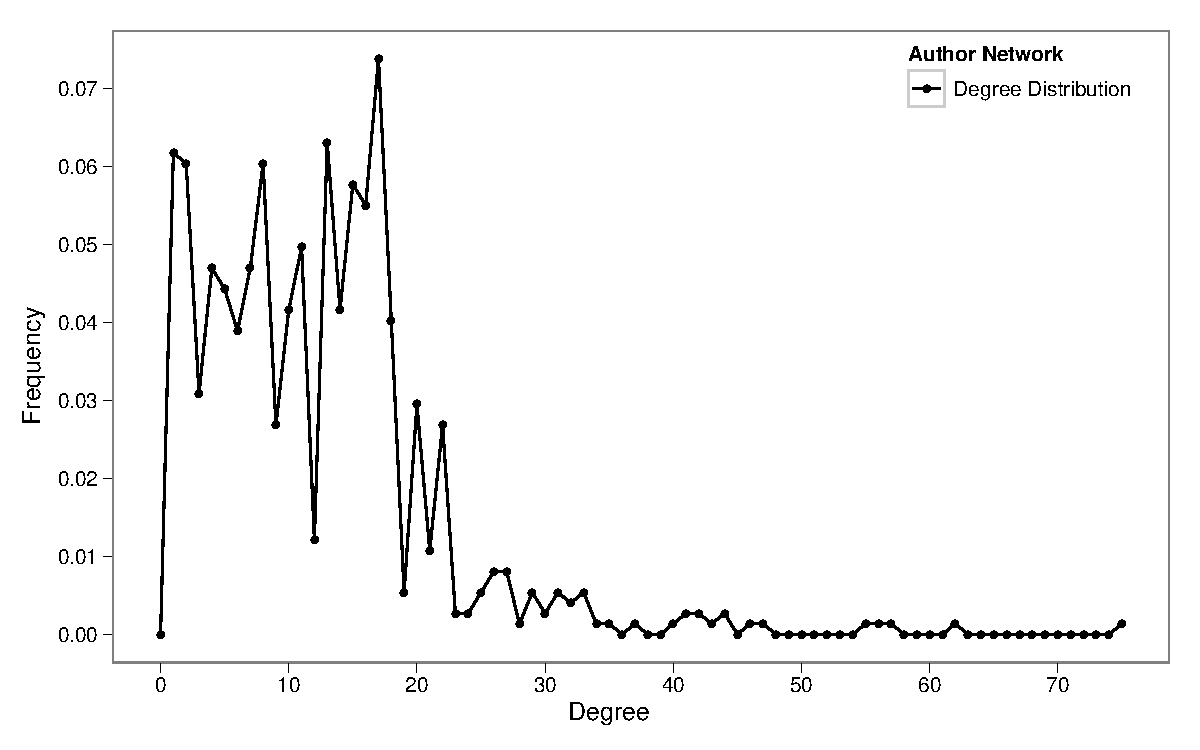
\includegraphics[width=10.5cm]{../images/authors_ddplot.pdf}
\end{frame}

\begin{frame}[fragile]
    \frametitle{Degree distributions}
    Articles \\
    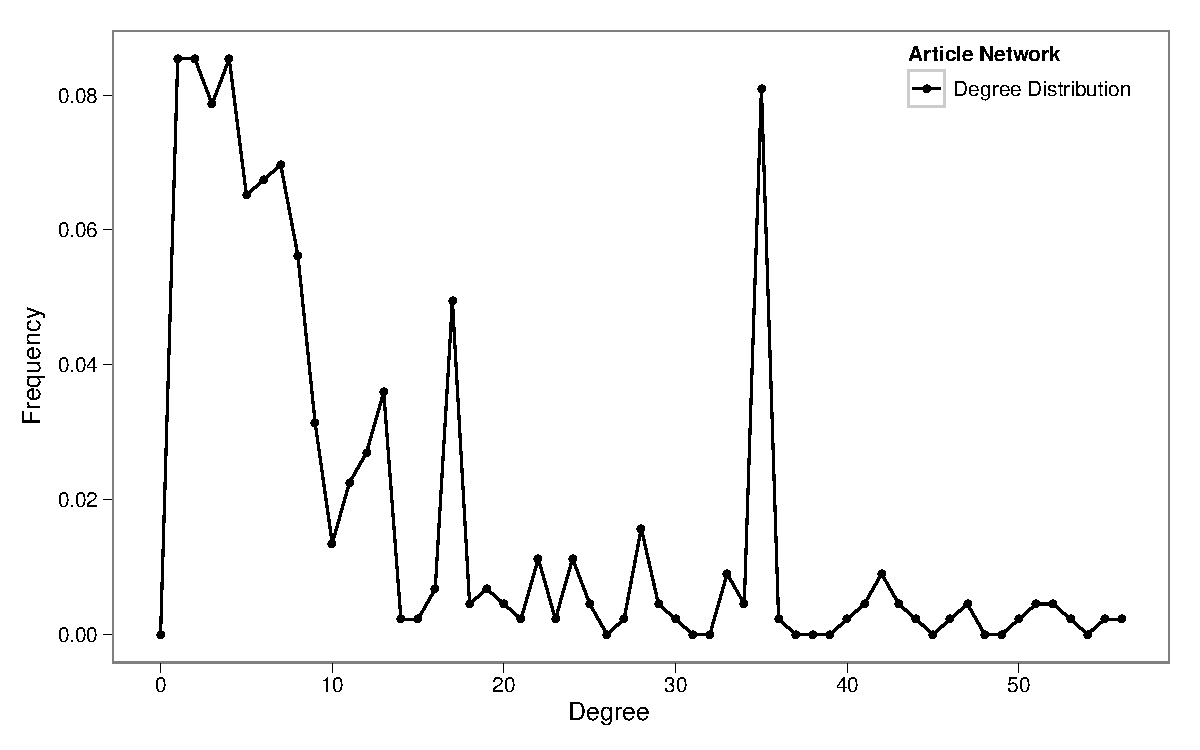
\includegraphics[width=10.5cm]{../images/articles_ddplot.pdf}
\end{frame}

\begin{frame}[fragile]
    \frametitle{Poisson fit}
    \begin{tabular}{l}
        Authors \\
        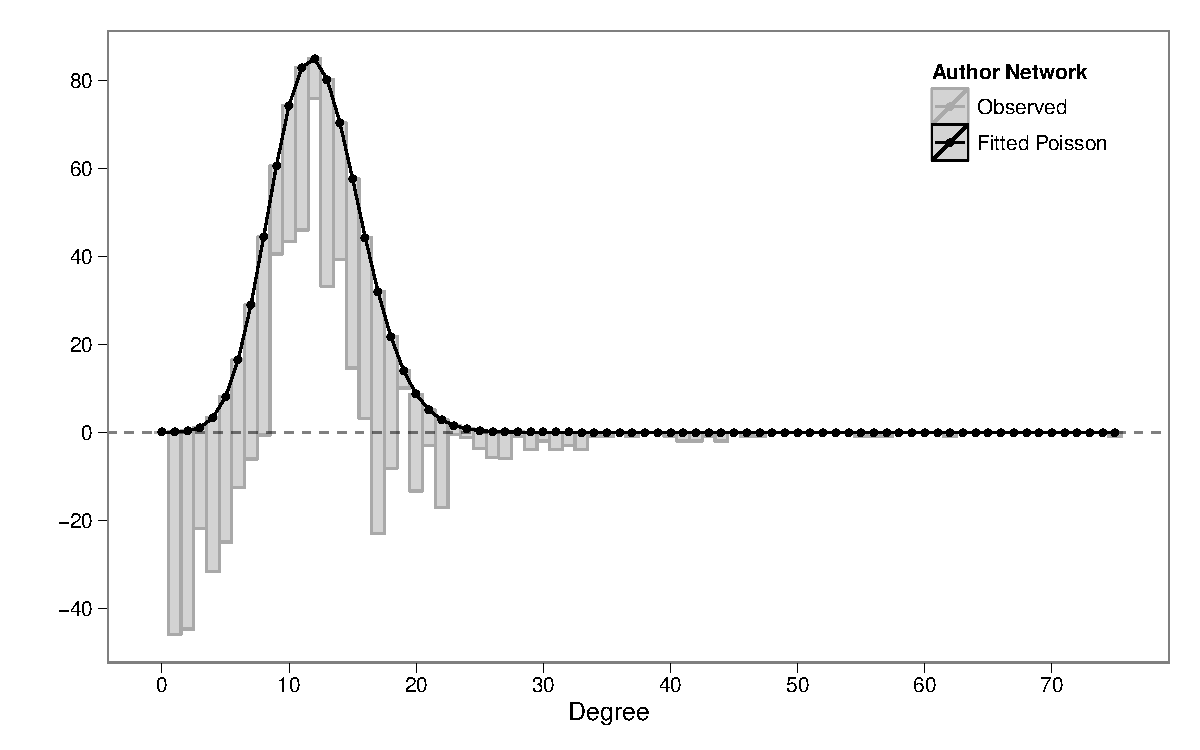
\includegraphics[width=10.5cm]{../images/authors_fitplot.pdf} \\
    \end{tabular}
    \begin{tabular}{ccc}
        $\lambda=12.06$ & $\chi^{2}=1760$ & p-value$=0.3509$
    \end{tabular}
\end{frame}

\begin{frame}[fragile]
    \frametitle{Poisson fit}
    \begin{tabular}{l}
        Articles \\
        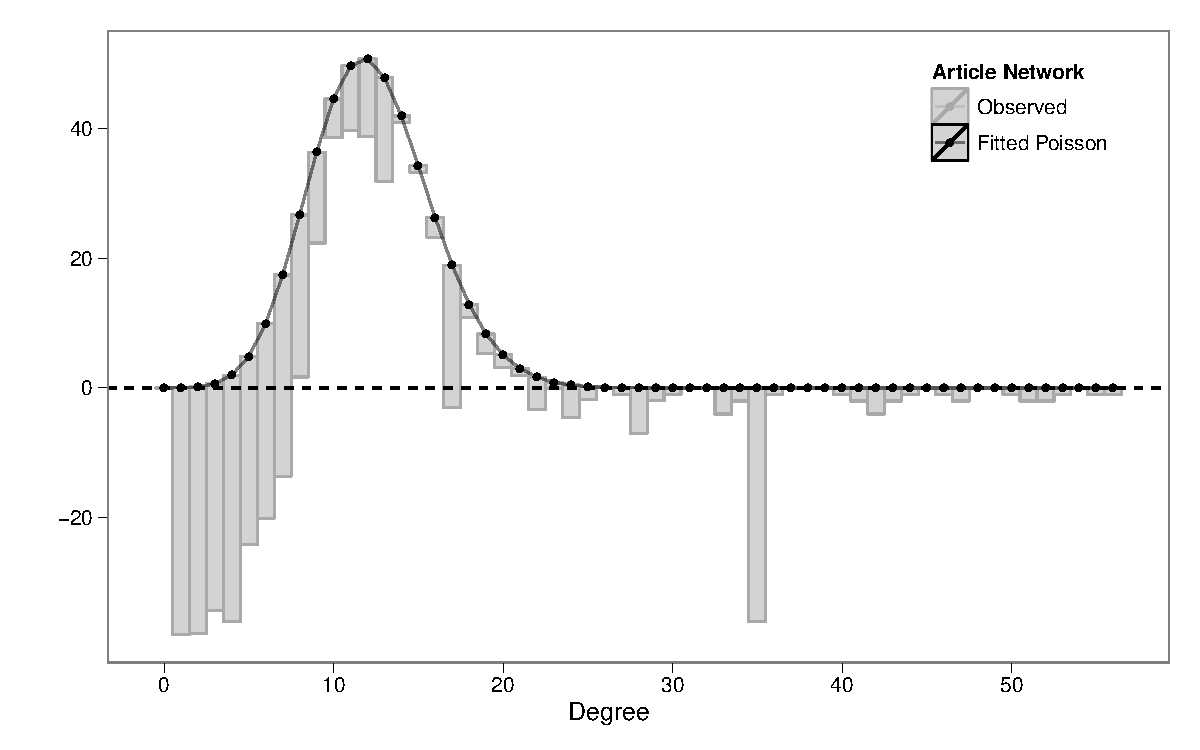
\includegraphics[width=10.5cm]{../images/articles_fitplot.pdf} \\
    \end{tabular}
    \begin{tabular}{ccc}
        $\lambda=11.70$ & $\chi^{2}=918$ & p-value$=0.3396$
    \end{tabular}
\end{frame}

\begin{frame}[fragile]
    \frametitle{Communities in article network}
        Does network structure reveal communities within Conflict Studies?
        \begin{itemize}
            \item What similarities exist among authors with similar structure?
            \item What topics are covered by articles with similar structure?
        \end{itemize}
        \uncover<2->{Community detection 
        \begin{itemize}
            \item Several methods exists
            \item Cottage industry in network science
            \item Use statistical method to determine partitions
            \item Block modeling
        \end{itemize}}
        \uncover<3->{Topic model of articles network
        \begin{itemize}
            \item Latent Dirichlet Allocation (LDA)
            \item Generate topics and terms
            \item Common and divergent themes?
        \end{itemize}}
\end{frame}

\begin{frame}[fragile]
    \frametitle{Visualizing communities in article network}
    \begin{center}
        \includegraphics[width=6cm]{../images/articles_spinglass_colored.pdf}
    \end{center}
\end{frame}

\begin{frame}[fragile]
    \frametitle{Articles block model}
    \begin{center}
        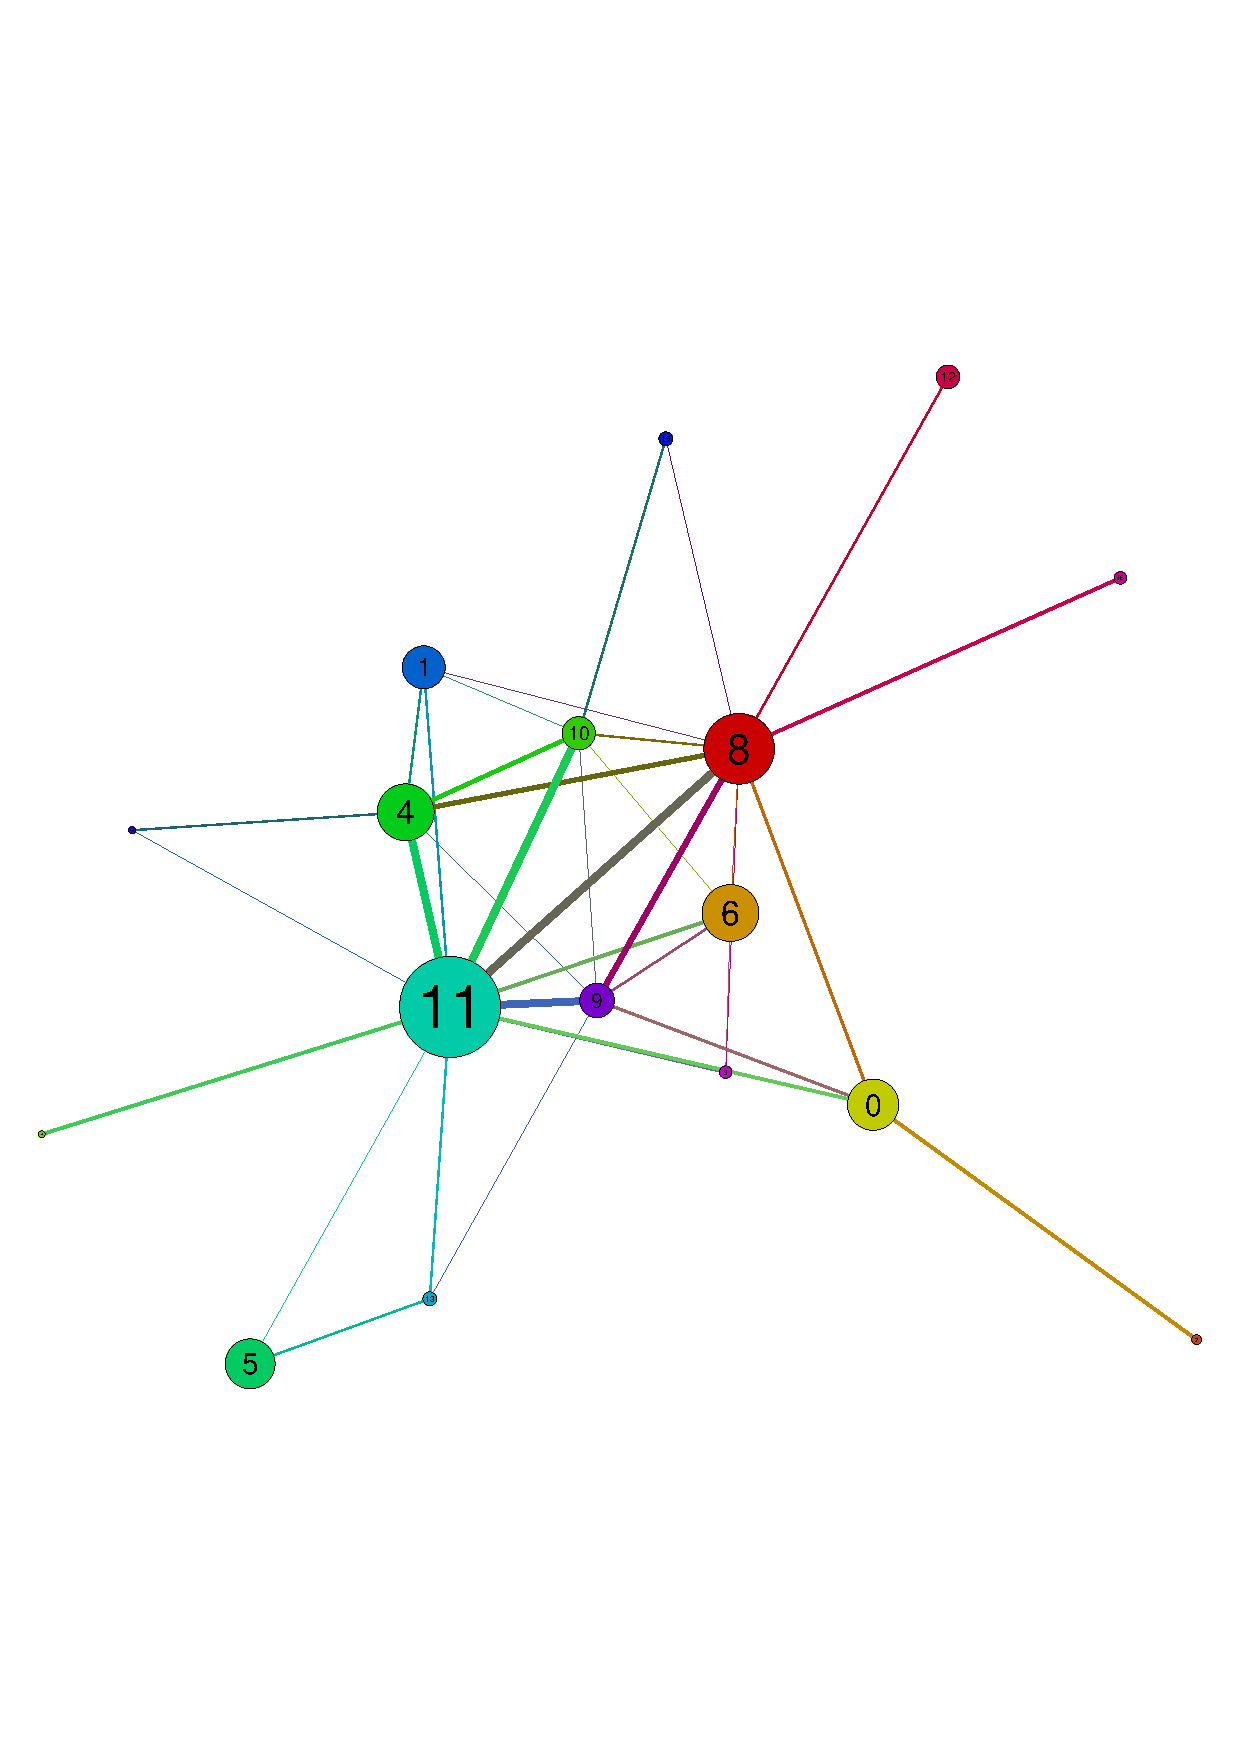
\includegraphics[width=7cm,clip,trim=0cm 4cm 0cm 4cm]{../images/articles_spinglass_blocked.pdf}
    \end{center}
\end{frame}

\begin{frame}[fragile]
    \frametitle{LDA topic models of partitions 4 \& 8}
        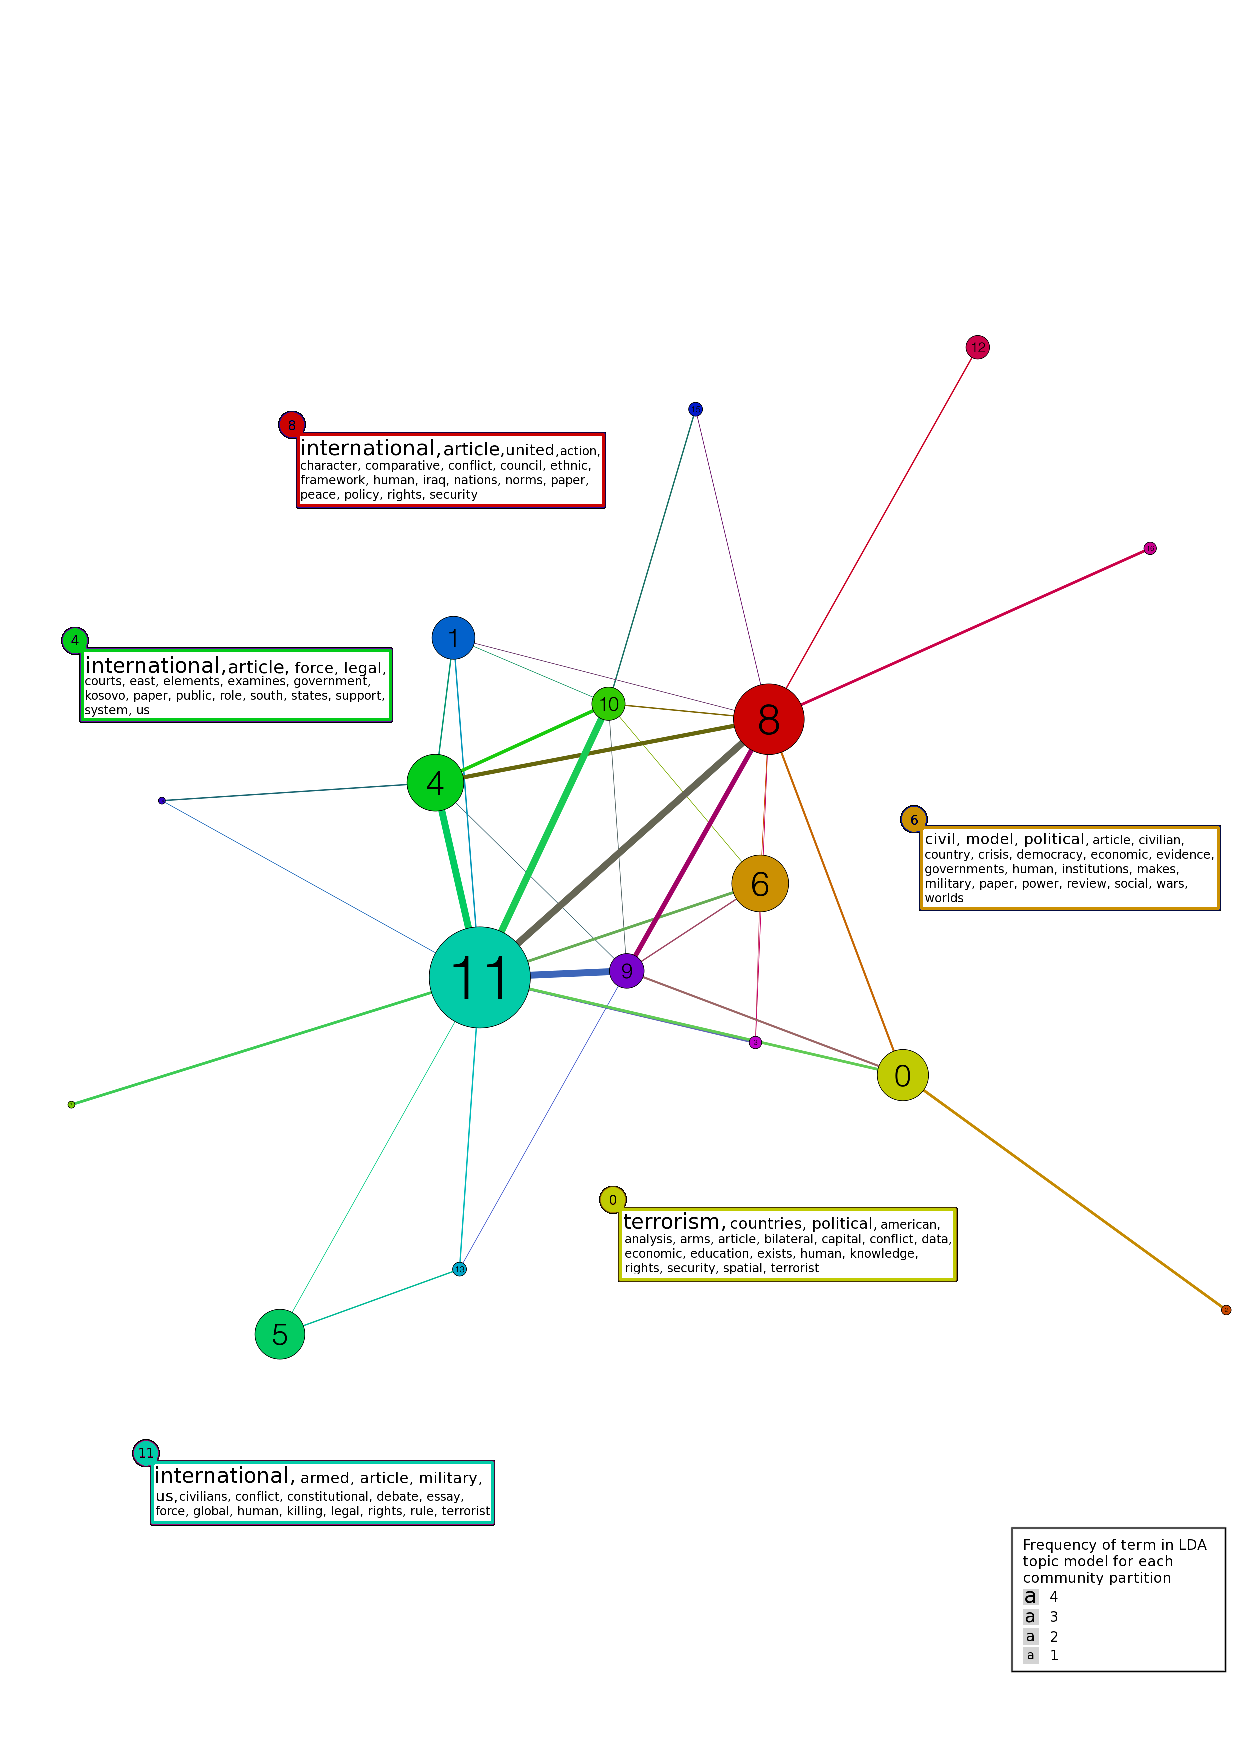
\includegraphics[width=15cm,clip,trim=1cm 4cm 2.5cm 3cm]{../images/articles_spinglass_topic_viz.pdf}
\end{frame}

\begin{frame}[fragile]
    \frametitle{LDA topic models of partitions 0, 6 \& 11}
    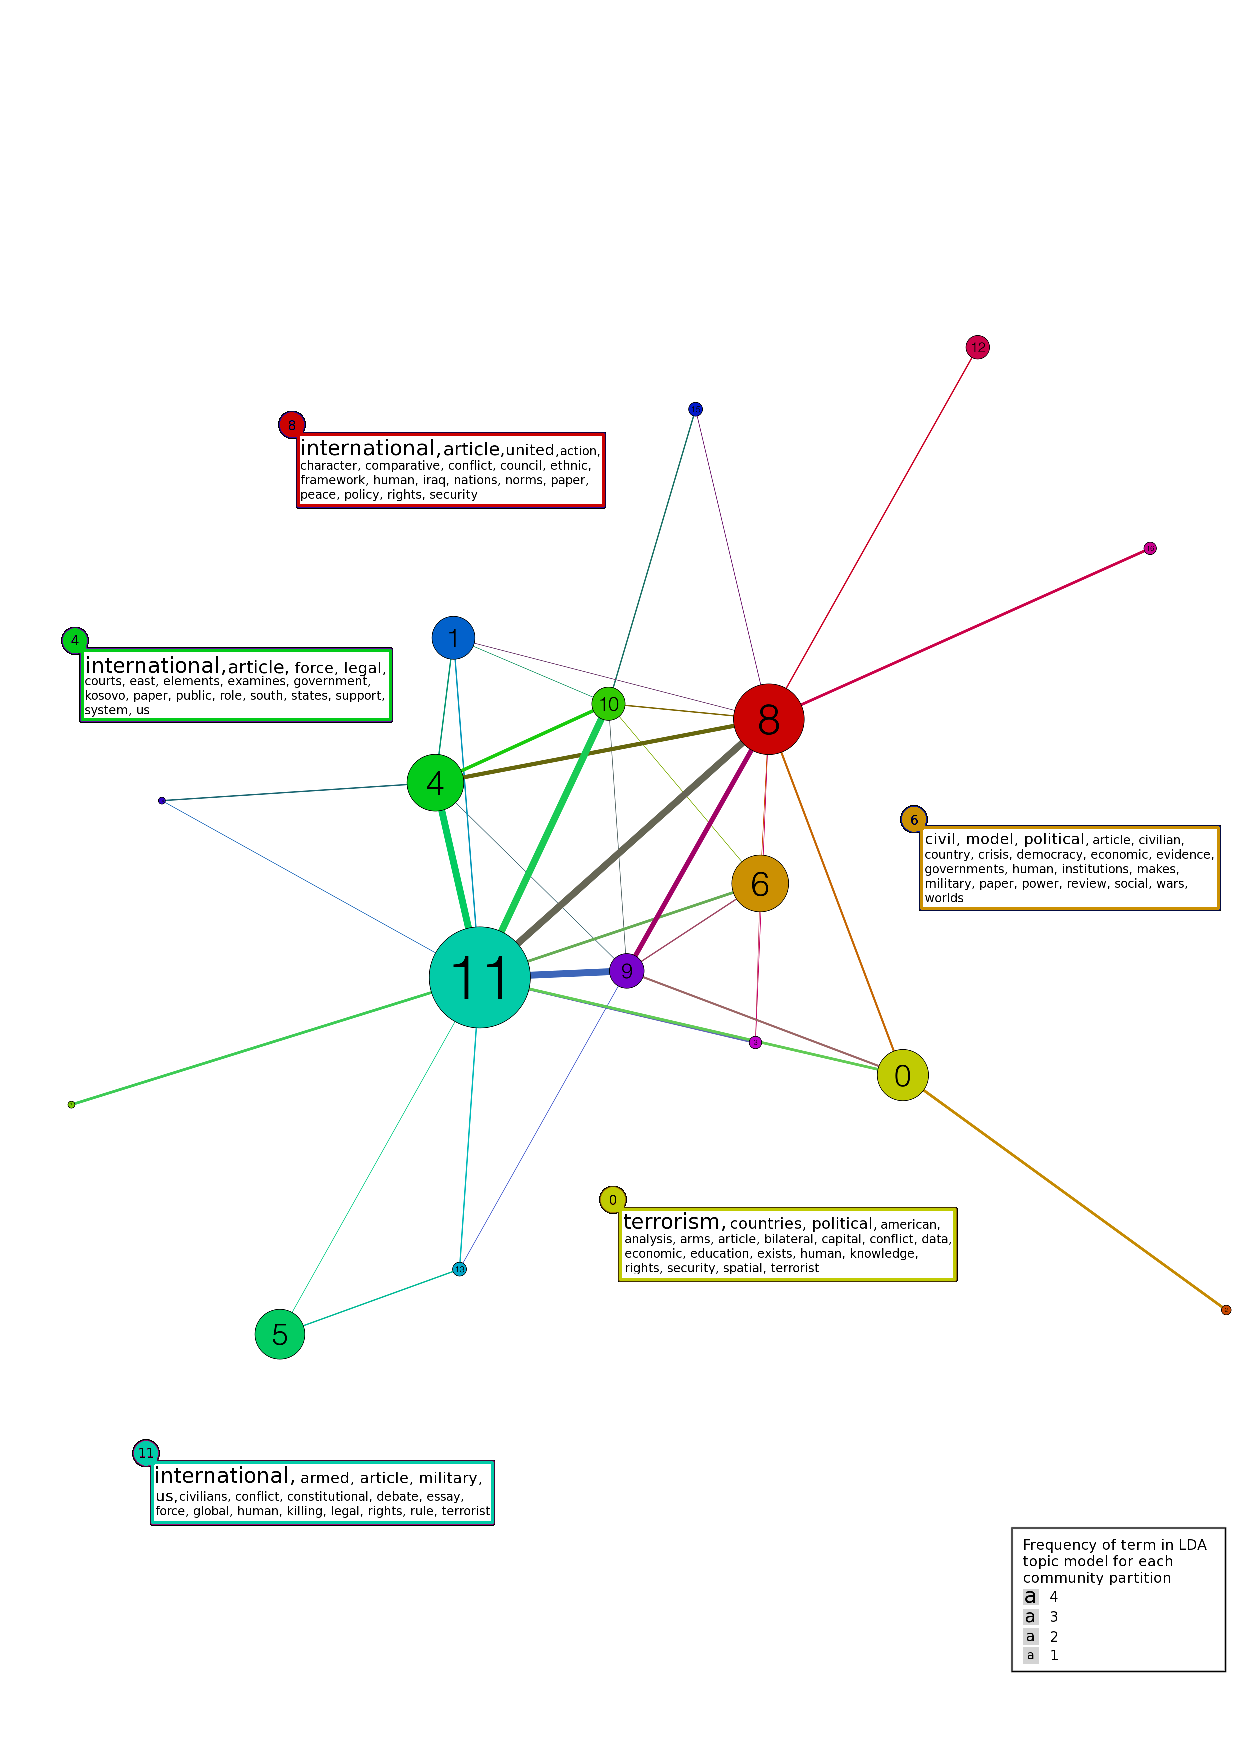
\includegraphics[width=12cm,clip,trim=2.1cm 0cm 0cm 11.6cm]{../images/articles_spinglass_topic_viz.pdf}
\end{frame}


% section analyzing_the_data (end)

\section{Network Economics} % (fold)
\label{sec:network_econonics}

\begin{frame}[fragile]
    \frametitle{Extending this research}
        Can this type of analysis be applied to economic networks?
        \begin{itemize}
            \item What would be the value?
            \item What contextual data would be worth collecting
            \item Additional analyses?
        \end{itemize}
        \begin{columns}
            \column{.33\textwidth}
            \uncover<2->{Venture Capital Investment
            \begin{itemize}
                \item Edges naturally temporal and weighted (frequency/amount)
                \item Structural communities vs. institutional
                \item Predict future co-investments
            \end{itemize}}
            \column{.33\textwidth}
            \uncover<3->{Nation state relationship
            \begin{itemize}
                \item Trade
                \item Defense 
                \item Evolution and/or decay
            \end{itemize}}
            \column{.33\textwidth}
            \uncover<4->{Market analysis
            \begin{itemize}
                \item Investor $\rightarrow$ security
                \item Market analysts $\rightarrow$ security
                \item Individuals $\rightarrow$ corporate governance
            \end{itemize}}
        \end{columns}
\end{frame}


% section network_econonics (end)

\end{document}
